\section{Results}
Our implementation comes with some tools that allow us to test and benchmark the implementation.
Each of these tools has been compiled with the flags \texttt{-mcpu=cortex-m4 -mthumb -ffunction-sections --fdata-sections -std=c99 -funroll-all-loops -pedantic -O3},
prioritizing the execution time more than the memory footprint.

\subsubsection*{\textbf{Functional testing}}
Before testing the performance of the scheme, we need to verify that the cryptosystem works as intended.
To check this, employ the same source code provided by the authors, checking that, when applying the KEM, the exchanged keys match.


\subsubsection*{\textbf{Execution time}}
In our benchmark we measure the execution time of the primitives of both the KEM and PKE schemes, as well as the multiplication.
To measure the number of clock cycles needed for each operation, we use the system timer. On a sample of 1000 runs, we get the following results:
\begin{figure}[H]
    \centering
    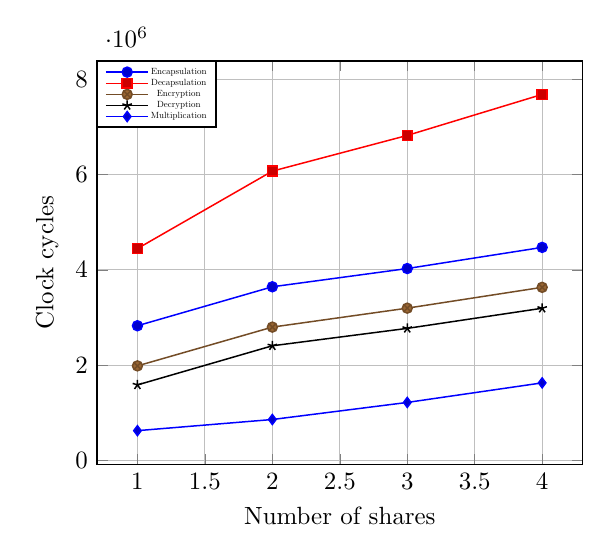
\begin{tikzpicture}[scale=0.9]
        \pgfplotsset{every axis/.append style={semithick}, legend style={at={(0,1)},anchor=north west, nodes={scale=0.6, transform shape}}}

	\begin{axis}[
		xlabel=Number of shares,ylabel=Clock cycles, grid=major,     x tick label style={
            /pgf/number format/.cd,
            precision=1,
        }]

    \addplot coordinates{
        (1, 2826067.47)
        (2, 3643555.40)
        (3, 4026514.86)
        (4, 4470225.81)

    };
    \addlegendentry{Encapsulation}

    \addplot coordinates{
        (1, 4445614.60)
        (2, 6070401.90)
        (3, 6819468.72)
        (4, 7680073.11)

    };
    \addlegendentry{Decapsulation}

    \addplot coordinates{
        (1, 1983894.79)
        (2, 2797433.27)
        (3, 3195107.26)
        (4, 3632298.13)

    };
    \addlegendentry{Encryption}

    \addplot coordinates{
        (1, 1584503.47)
        (2, 2405541.52)
        (3, 2770976.91)
        (4, 3193077.76)

    };
    \addlegendentry{Decryption}

    \addplot coordinates{
        (1, 624965.27)
        (2, 858842.66)
        (3, 1216993.20)
        (4, 1627512.25)

    };
    \addlegendentry{Multiplication}
    \end{axis}%
\end{tikzpicture}%
\caption{Execution time (clock cycles)}
\end{figure}
\begin{table}[H]
    \begin{tabular}{llllll}
        \# & encaps & decaps & enc & dec & mul \\ \hline
        2 & 28.92 & 36.55 & 41.00 & 51.81 & 37.42 \\
        3 & 42.48 & 53.40 & 61.05 & 74.88 & 94.73 \\
        4 & 58.18 & 72.76 & 83.09 & 101.51 & 160.41
    \end{tabular}
    \caption{Percentual performance decrease}
\end{table}
As we can observe, the overhead factor introduced by the masking operations is less than 2 for any operation, 
unlike the results obtained for some other cryptosystems (\cite{belaid:hal-02953167,cryptoeprint:2020:733,cryptoeprint:2021:483})

\newpage

\subsubsection*{Constant-time execution}
To detect an eventual leakage we rely on the \textit{t-test}-based Test Vector Leakage Assessment (TVLA, \cite{schneider2015leakage}): 
we compare the measurements between two populations (fixed \textit{vs} random) of 1000 samples each, and affirm that there is no correlation
between the two if $|t| < 4.5$.

For both primitives we precompute keypair and secret message for the fixed measurements, while generating fresh randomness for the masks; we then measure 
the execution time as for the timing test, and obtain the following results:

\begin{table}[H]
    \begin{tabular}{llllll}
        \# & encaps & decaps & enc & dec & mul \\ \hline
        1 & 0.93666 & 4.56649 & 25.66178 & 10.26449 & 30.09420 \\
        2 & 6.00482 & 3.35650 & 4.62100 & 5.96089 & 4.96460 \\
        3 & 0.28901 & 1.69393 & 1.59911 & 5.88290 & 3.50812 \\
        4 & 0.12693 & NA & 3.30161 & 4.01299 & 0.21834
    \end{tabular}
    \caption{Welch's t (abs. value)}
\end{table}

We can note how the values tend to decrease for the KEM, PKE and multiplication, hinting that
by applying masking mechanisms of increasing order the information leakage decreases. There are some anomalies in this trend
that might be caused by a \textit{bad} initialization of the PRNG; this should be investigated by repeating the tests on a 
similar board equipped with a TRNG.





